\documentclass[../main.tex]{subfiles}
\begin{document}
\chapter{Reading of This Book}
\section{Structures}
I summarize the characteristics that potentially set this book apart from other books seen in the market; starting from introducing technically what I think of the core principles of algorithm design are--the ``source'' of the wisdom I was after as mentioned in the preface, to illustrating the concise organization of the content, and to highlighting other unique features of this book. 
\subsubsection{Core Principles}
Algorithm problem solving follows a few core principles: Search and Combinatorics, Reduce and Conquer, Optimization via Space-Time Trade--off or be Greedy. We specifically put these principles in one single part of the book--Part.~\ref{part_core_principles}.
\begin{enumerate}
    \item In Chapter.~\ref{chapter_search_problem_combinatorics} (Search and Combinatorics), I teach how to formulate problems as searching problems via combinatorics in the field of math to enumerate its state space—solution space or all possibilities. Then we further optimize and improve the efficiency through ``backtracking'' techniques. 
\item In Chapter.~\ref{chapter_divide_and_conquer}(Reduce and Conquer) we can either reduce problem A to problem B (solving problem B means we solved problem A)  or Self-Reduction to reduce problem to a series of subproblems (Such as these algorithm design methodologies fall into this area:  divide and conquer, some search algorithms, dynamic programming and greedy algorithms). \textbf{Mathematical induction} and \textbf{recurrence relations} play as an important role in  problem solving, complexity analysis and even correctness proof.  
\item When optimization is needed, we have potentially two methods: 
when we see the subproblems/states overlap, space-time trade-off can be applied such as in dynamic programming;
Or we can make greedy choice based on current situation. 
\end{enumerate}
\subsubsection{Concise and Clear Organization}
\begin{figure}[h]
    \centering
    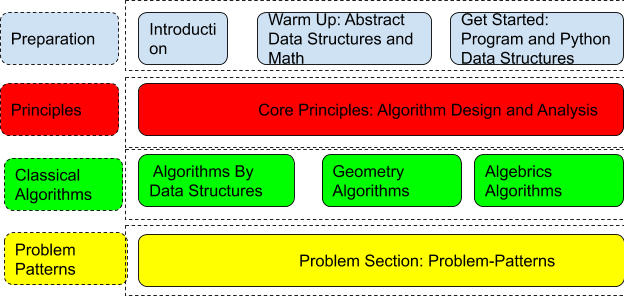
\includegraphics[width=1\columnwidth]{fig/four_umbreallas.png}
    \caption{Four umbrellas:  each row indicates corresponding parts as outlined in this book.}
    \label{fig:four_umbreallas}
\end{figure}

In this book, we organize in the ordering of Part, Chapter, Section, Subsection, Subsubsection and Paragraph. The parts will be categorized under four umbrellas and each serves an essential purpose: 
\begin{enumerate}
    \item Preparation: Introduce the global picture of algorithmic problem solving and coding interviews, learn abstract data structures and highly related and useful math such as recurrence relation, and hands-on Python practice by relating the abstract data structures to Python data structures. 
\item Principles: As we introduced in the core principle part, we organize the design and principle here so that readers can use them as guidance while not seeking for peculiar algorithm for solving a problem. 
\item Classical algorithms: We enhance our algorithm database via learning how to apply the core principles to a variety of classical problems. A database that we can quickly relate to when seeing problems. 
\item Coding interview problem patterns:  We close our book with the analyzing and categorizing problems by patterns. We address classical and best solutions for each problem pattern. 
\end{enumerate}
\subsubsection{Other Features and Uniqueness}
\begin{enumerate}
    \item The exercise and answer setting: at the problem-pattern section, the first chapter will be named problem pool which list all problems with description. At each exercise section across chapters, only problem id is referred. Instead the answers to problems are organized by different patterns so that users can review problem solving skills quickly when preparing for an interview.This is also practical to problem solving skills. 
\item Real coding interview problems referred from LeetCode,  users can easily practice online and join discussions with other users.
\item Real Python Code included in the textbook and offered via Google Colab instead of using Pseudo-code. 
\item The content is grain-scaled, great for users to skim when necessary to prepare for interviews. 
\item Included practical algorithms that are extremely useful for solving coding interview problems and yet are almost never be included in other books, such as monotone stack, two-pointer techniques, and bit manipulation with Python. 
\item Included highly related math methods to ease the learning of the topic, including recurrence relations, math formulas, math induction method. 
\item Explanation of concepts are problem solving oriented, this makes it easier for users to grasp the concepts. We introduce the concepts along with examples, we strengthen and formalize the concepts in the summary section.
\end{enumerate}

\subsubsection{Q \& A} 
\paragraph{What do we not cover?} In the spectrum of coding interviews and the spectrum of the algorithms, we do not include:
\begin{itemize}
    \item Although this book is a comprehensive combination of Algorithmic Problem Solving and Coding Interview Coaching, I decided not to provide preparation guideline to the topic of \textbf{System Design} to avoid deviation from our main topic. An additional reason is, personally, I have no experience yet about this topic and meanwhile it is not a topic that I am currently interested in either, so a better option is to look for that in another book. 
\item On the algorithm side, we briefly explain what is \textbf{approximate algorithms}, \textbf{heuristic search}, and linear programming, which is mainly seen in Artificial Intelligence, such as machine learning algorithms and neural networks. We do mention it because I think it is important to know that the field of artificial intelligence are just simply a subfield of algorithms, it is powerful because of its high dimensional modeling and large amount of training data. 

\end{itemize}
\paragraph{How much we include about Python 3? } We use Python 3 as our programming language to demonstrate the algorithms for its high readability and popularity in both industry and academics. We mainly focus on Python built-in Data types, frequently used modules, and a single class, and leave out knowledge such as object-oriented programming that deals with class heritages and composition, exception handling, an so on. Our approach is to provide brief introduction to any prior Python 3 knowledge when it is first used in the book, and put slightly more details in the Appendix for further reading and reference. We follow PEP 8 Python programming style. If you want to the object-oriented programming in Python, Python 3 Object-oriented programming is a good book to use. 

\paragraph{Problem Setting} Compared with other books that talk about the problem solving (e.g. \textit{Problem Solving with Algorithms and Data Structures}, we do not talk about problems in complex setting. We want the audience to have a simple setting so that they can focus more on analyzing the algorithm or data structures' behaviors.  This way, we keep out code clean and it also serves the purpose of coding interview in which interviewees are required to write simpler and less code compared with a real engineering problems because of the time limit. 


Therefore, the purpose of this book is three-fold: to answer your questions about interview process, prepare you fully for the ``coding intervie'', and the most importantly master algorithm design and analysis principles and sense the beauty of them and in the future to use them in your work. 

\section{Reading Suggestions}
We divide the learning of this book in four stages, each stage builds up on each other. Evaluate which stage you are, and we kindly suggest you to read in these orders: 
\begin{itemize}
    \item \textbf{First Stage} I recommend readers first start with Part Two, fundamental algorithm design and analysis, part Three, bit manipulation and data structures to know the basics in both algorithm design and data structures. In this stage, for graph data structures, we learn BFS and DFS with their corresponding properties to help us understand more graph and tree based algorithms. Also, DFS is a good example of recursive programming. 
\item \textbf{Second Stage}
In the second stage, we move further to Part Four, Complete Search and Part Five, Advanced Algorithm Design. The purpose of this stage is to move further to learn more advanced algorithm design methodologies: universal search, dynamic programming, and greedy algorithms. At the end, we will understand under what condition, we can improve our algorithms with efficiency from searching-based algorithms to dynamic programming, and similarly from dynamic programming to greedy algorithms. 
\item \textbf{Third Stage}
After we know and practiced the universal algorithm design and know their difference and handle their basic problems. We can move to the third stage, where we push ourselves further in algorithms, we learn more advanced and special topics which can be very helpful in our career. The content is in Part Six, Advanced and  Special Topics. 
\begin{enumerate}
    \item For example, we learn move advanced graph algorithms. They can be either BFS or DFS based. 
    \item Dynamic programming special, where we explore different types of dynamic programming problems to gain even better understanding to this topic.
    \item String pattern Matching Special: 
\end{enumerate}

\item \textbf{Fourth Stage}
In this stage, I recommend audience to review the content by topics:
\begin{enumerate}
    \item Graph: Chapter Graphs, Chapter Non-linear Recursive Backtracking, Chapter Advanced Graph Algorithms, Chapter Graph Questions. 
    \item Tree: Chapter Trees, Chapter Tree Questions
    \item String matching: Chapter String Pattern Matching Special, Chapter String Questions
    \item Other topics: Chapter Complete Search, Chapter Array Questions, Chapter Linked List, Stack, Queue and Heap. 
\end{enumerate}
\end{itemize}

\subsubsection{Wanna Finish the Book ASAP? Or just review it for interviews?}  I organize the book in all of forty chapters, it is a lot but they are carefully put under different parts to highlight each individual's purpose in the book. We can skim difficult chapters marked by asterisk($*$) that will unlikely appear in a short-time interview. The grained categorization helps us to skim on the chapter levels, if you are confident enough with some chapters or you think they are too trivial, just skim, given that the book is designed to be self-contained of multiple fields(programming languages, algorithmic problem solving and the coding interview problem patterns). 

The content within the book is almost always partitioned into paragraphs with titles. This conveniently allows us to skip parts that are just for enhancement purpose, such as ``stores'' or . This helps us skim within each chapter. 
\end{document}